\documentclass[landscape]{slides}
\usepackage[landscape, margin=2cm]{geometry}
\usepackage{color}
\usepackage{bm}
\usepackage{graphicx}
\usepackage{hyperref}
\usepackage{soul}
\graphicspath{ {./img/} }



\title{Sleep}
\author{Adam Johnson}
\date{30th April 2014}

\begin{document}

\maketitle


\begin{slide}

    \textcolor{blue}{\Large{Let's start with a personality quiz...}}

    \small{Source: ``Night School'' - Richard Wiseman, 2014}

\end{slide}


\begin{slide}

    \textcolor{blue}{\Large{1) If you were free to plan your evening, and had no commitments the next day, what time would you choose to go to bed?}}

    \begin{enumerate}
        \item Before 21.00
        \item 21.00 - 22.30
        \item 22.30 - 00.00
        \item 00.00 - 01.30
        \item After 1.30
    \end{enumerate}

\end{slide}


\begin{slide}

    \textcolor{blue}{\Large{2) If you were free to plan your day, what time would choose to get up?}}

    \begin{enumerate}
        \item Before 06.30
        \item 06.30 - 08.00
        \item 08.00 - 09.30
        \item 09.300 - 11.00
        \item After 11.00
    \end{enumerate}

\end{slide}



\begin{slide}

    \textcolor{blue}{\Large{3) In general, do you find it easy to get up in the morning?}}

    \begin{enumerate}
        \item Definitely yes
        \item Yes
        \item Uncertain
        \item No
        \item Definitely no
    \end{enumerate}

\end{slide}



\begin{slide}

    \textcolor{blue}{\Large{4) Imagine that you have to do two hours of physically hard work. If you were entirely free to plan your day, in which of the following periods would you choose to do the work?}}

    \begin{enumerate}
        \item 08.00 - 11.00
        \item 11.00 - 13.00
        \item 13.00 - 15.00
        \item 15.00 - 17.00
        \item 17.00 - 19.00
    \end{enumerate}

\end{slide}



\begin{slide}

    \textcolor{blue}{\Large{Results...}}

\end{slide}


\begin{slide}

    \textcolor{blue}{\Large{Your Chronotype}}

    \begin{tabular}{c | c | c | c | c}

        4 - 6 &
        7 - 10 &
        11 - 13 &
        14 - 17 &
        18 - 20 \\

        \parbox[t]{4.2cm}{
            \begin{center}
            \textbf{Strong lark}
            \end{center}
        } &
        \parbox[t]{4.2cm}{
            \begin{center}
            \textbf{Moderate lark}
            \end{center}
        } &
        \parbox[t]{4.2cm}{
            \begin{center}
            \textbf{Neither owl nor lark}
            \end{center}
        } &
        \parbox[t]{4.2cm}{
            \begin{center}
            \textbf{Moderate owl}
            \end{center}
        } &
        \parbox[t]{4.2cm}{
            \begin{center}
            \textbf{Strong owl}
            \end{center}
        } \\

        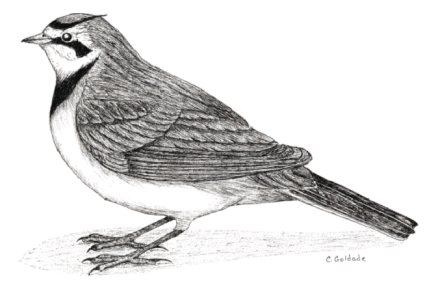
\includegraphics[width=4.2cm]{lark} &
        & & &
        
\includegraphics[width=4.2cm]{owl} \\

    \end{tabular}

\end{slide}



\begin{slide}

    \textcolor{blue}{\Large{What does your chronotype say about your personality?}}

    \textbf{Larks:}

    \begin{itemize}
        \item introverted, logical, and reliable
        \item get higher grades
    \end{itemize}

    \textbf{Owls:}

    \begin{itemize}
        \item extroverted, emotionally stable, hedonistic, and creative
        \item more likely to be obese
        \item average of four times as many partners during lifetime
    \end{itemize}

\end{slide}


\begin{slide}

    \textcolor{blue}{\Large{...so what about my sleep-improving habits?}}

\end{slide}


\begin{slide}

    \textcolor{blue}{\Large{1. Go to bed alarm}}

    \begin{center}
        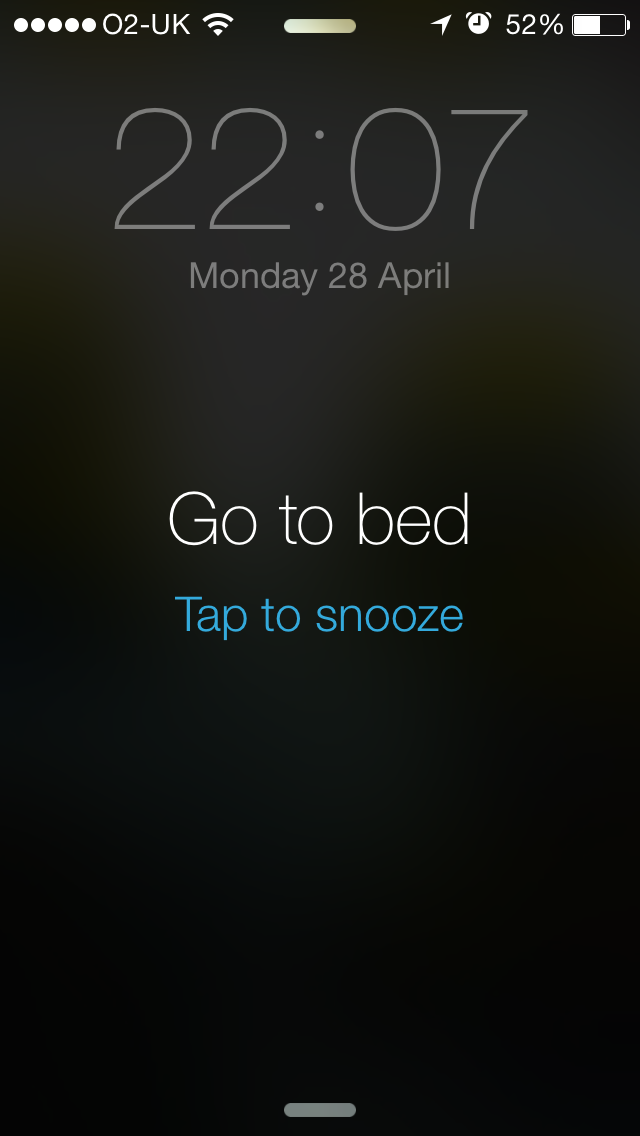
\includegraphics[height=15.5cm]{go-to-bed-alarm}
    \end{center}

\end{slide}


\begin{slide}

    \textcolor{blue}{\Large{2. Melatonin Supplement}}

    \begin{itemize}
        \item Mammalian sleep hormone
        \item Strong evidence that everyone in the Western world has much lower levels of it
        \item 1.5mg nightly, at 10pm when alarm goes
    \end{itemize}

    \small{Ref: \url{http://www.gwern.net/Melatonin}}

\end{slide}


\begin{slide}

    \textcolor{blue}{\Large{3. Yellow Glasses}}

    \begin{center}
        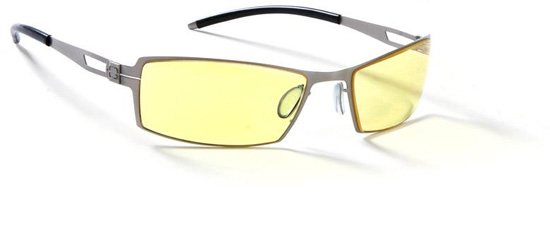
\includegraphics[height=10cm]{gunnars}
    \end{center}

    \begin{itemize}
        \item Not stylish, but they work
    \end{itemize}

\end{slide}


\begin{slide}

    \textcolor{blue}{\Large{4. F.lux}}

    \begin{center}
        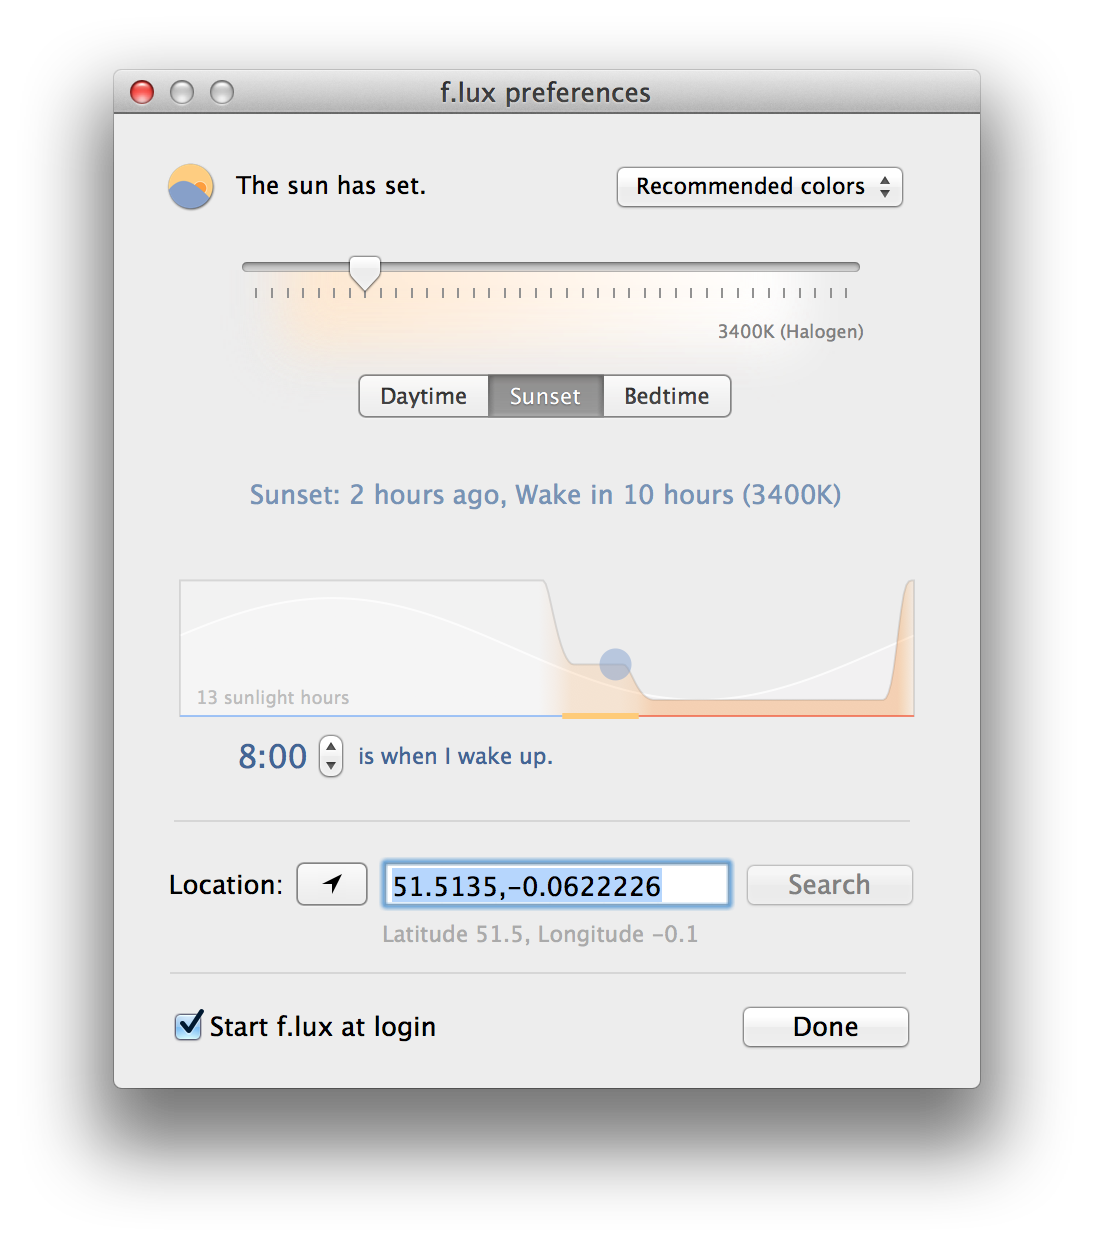
\includegraphics[height=12cm]{flux}
    \end{center}

    \begin{itemize}
        \item \url{https://justgetflux.com/}
    \end{itemize}

\end{slide}


\begin{slide}

    \textcolor{blue}{\Large{5. Napping}}

    \begin{center}
        
\includegraphics[height=10cm]{dog-napping}
    \end{center}

    \begin{itemize}
        \item Really good for learning...
    \end{itemize}

\end{slide}


\begin{slide}

    \textcolor{blue}{\Large{5. Napping}}

    \begin{quote}
        ``Practice is often believed to be the only determinate of improvement. Although repeatedly performing a new task often results in learning benefits, leading to the adage ``practice makes perfect,'' a collection of studies over the past decade has begun to change this concept. Instead, these reports suggest that after initial training, \hl{the human brain continues to learn in the absence of further practice, and that this delayed improvement develops during sleep.}''
    \end{quote}

    \small{Source: ``It's Practice, with Sleep, That Makes Perfect: Implications of Sleep-Dependent Learning and Plasticity for Skill Performance'' - Walker and Stickgold, 2005}

\end{slide}


\begin{slide}

    \textcolor{blue}{\Large{5. Napping}}

    \begin{quote}
        ``These findings suggest that \hl{the 10-minute nap was overall the most effective afternoon nap duration} of the nap lengths examined in this study.''
    \end{quote}

    \small{Source: ``A Brief Afternoon Nap Following Nocturnal Sleep Restriction: Which Nap Duration is Most Recuperative?'' - Brooks and Lack, 2006}

\end{slide}


\begin{slide}

    \textcolor{blue}{\Large{Thanks!}}

    \begin{center}
        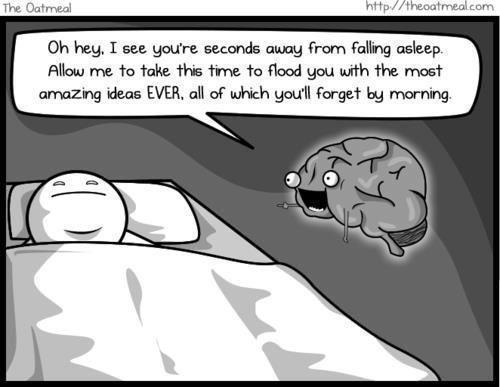
\includegraphics[height=15.5cm]{oatmeal-sleep-brain}
    \end{center}

\end{slide}


\end{document}
